\chapter{CÁC KIẾN THỨC NỀN TẢNG}

	\fontsize{12pt}{7pt}\selectfont
	\noindent\textit{Chương này sẽ giới thiệu một cách tổng quan về E-Learning, chuẩn SCORM và công cụ đọc nội dung theo chuẩn SCORM. Tiếp theo sẽ trình bày công cụ eXe Learning được lựa chọn để phát triển, bao gồm các công nghệ được sử dụng, kiến trúc hệ thống cũng như kiến trúc phần mềm của nó. Cuối cùng sẽ giới thiệu công cụ kiểm thử tự động được dùng để kiểm thử các chức năng của eXe.}


\section{Giới thiệu về E-Learning}
	Cùng với sự phát triển lớn mạnh của công nghệ thông tin, việc dạy và học truyền thống cũng đã có những thay đổi lớn nhờ vào việc ứng dụng công nghệ E-Learning vào trong việc dạy và học. E-Learning là một công nghệ mới, với nhiều ưu điểm so với học tập truyền thống. Trong những năm 2000, các doanh nghiệp lớn trên thế giới đã ứng dụng E-Learning để đào tạo nhân viên của họ, E-Learning giúp tạo một hệ thống thông tin tương tác cao giữa các nhân viên, giúp họ dễ dàng trao đổi để nâng cao nghiệp vụ của mình. Ngày nay, E-Learning được ứng dụng rộng rãi trong hệ thống đào tạo tại các trường đại học và các trung tâm đào tạo lớn.\\

	E-Learning(Giáo dục trực tuyến) là một hình thức học tập thông qua mạng Internet dưới dạng các khóa học và được quản lý bởi các hệ thống quản lý học tập, nhằm đảm bảo sự tương tác, hợp tác và đáp ứng nhu cầu học mọi lúc, mọi nơi của người học. Khác với các phương pháp học tập truyền thống, người học sẽ được truyền tải kiến thức thông qua nội dung được các giảng viên xây dựng, biên soạn sẵn. Các nội dung truyền đạt kiến thức được thể hiện bằng nhiều hình thức khác nhau như video, hình ảnh, bài tập vận dụng,... Bên cạnh đó E-Learning cũng cung cấp một môi trường học tập tương tác cao như diễn đàn, nhóm trao đổi hay các bài tập đánh giá,...\\

	Mở rộng ra, các cá nhân hay tổ chức đều có thể tự lập ra một trường học trực tuyến(E-School) để nhận đào tạo học viên, đóng học phí, có các bài kiểm tra và được cấp chứng nhận sau khi hoàn thành khóa học như một trường học truyền thống. Một số trường học trực tuyến phổ biến hiện nay có số lượng học viên lớn như Udemy, Edumall, hocmai.vn,... Phần lớn các trường đại học trên thế giới nói chung hay Việt Nam nói riêng đều có hệ thống E-Learning để phục vụ tốt hơn cho việc dạy và học của giảng viên và sinh viên. E-Learning đã thay đổi hoàn toàn phương pháp học tập truyền thống, phần sau đây sẽ trình bày một số ưu điểm và nhược điểm của việc sử dụng hệ thống E-Learning trong giáo dục.

\newpage

\subsection{Ưu điểm của E-Learning so với học tập truyền thống}

	Mặc dù không thể thay thế hoàn toàn phương pháp học tập truyền thống nhưng E-Learning phần nào cũng đã khắc phục, củng cố những hạn chế của phương pháp học tập truyền thống. Một số ưu điểm của E-Learning có thể kể đến như:

	\begin{itemize}
		
		\item \textbf{Tiết kiệm chi phi đào tạo:} Nội dung của bài giảng E-Learning có thể sử dụng cho nhiều khóa học khác nhau nên có thể tiết kiệm được từ 40\% đến 60\% chi phí đào tạo so với hình thức đào tạo truyền thống.
	
		\item \textbf{Độ linh hoạt cao:} Học viên sẽ không bị giới hạn bởi không gian và thời gian. Chỉ cần có một đường truyền Internet là học viên có thể tiến hành học ở bất cứ đâu và bất cứ lúc nào.
	
		\item \textbf{Tính tương tác cao:} Sự hỗ trợ mạnh mẽ của các đa phương tiện như hình ảnh, âm thanh, hoạt hình hay các công cụ giả lập,... giúp cho bài học sinh động hơn, cuốn hút hơn và cũng dễ hiểu hơn.
	
		\item \textbf{Tính chủ động cao:} E-Learning chủ yếu dựa trên tính chủ động của người học. Thậm chí có một số quan điểm xem E-Learning là việc ứng dụng công nghệ để hỗ trợ cho việc tự học. Người dùng ngoài việc chủ động chọn khóa học, nội dung và thời gian, còn có thể tự đánh giá khả năng của mình qua các bài kiểm tra của nội dung đó để bảo đảm có được lượng kiến thức cần thiết trước khi chuyển sang nội dung khác. Người học cũng có thể theo dõi tiến độ học tập của mình nhờ vào những công cụ quản lý của hệ thống E-Learning.
	
		\item \textbf{Tính mở rộng cao:} Với sự giúp đỡ của các trình soạn thảo nội dung hiện nay thì việc thiết kế một bài giảng có các nội dung phong phú, bài tập đa dạng,... là hoàn toàn có thể thực hiện được.
	
	\end{itemize}


\subsection{Nhược điểm của E-Learning}
	
	Những hạn chế của phương pháp học tập trực tuyến(E-Learning) so với phương pháp học tập truyền thống có thể kể đến như sau:

	\begin{itemize}
		
		\item \textbf{Giảm khả năng giao tiếp:} Dù nội dung bài học có sinh động, phong phú đến đâu cũng sẽ không tốt bằng sự chỉ bảo tận tình của giảng viên. Việc chỉ áp dụng học trực tuyến sẽ khiến người học khó kết giao bạn bè, đồng thời cũng hạn chế sự giao tiếp với bên ngoài.
	
		\item \textbf{Không tạo được môi trường học tập tích cực chủ động:} Người học chủ yếu học được kiến thức nhưng không học được cách vận dụng những kiến thức đó một cách thực tế. Ngoài ra người học còn bị hạn chế phát triển một số kỹ năng đòi hỏi tính tương tác cộng đồng cao như kỹ năng làm việc nhóm, kỹ năng thuyết trình,...
	
		\item \textbf{Dễ gây mất tập trung:} Việc ngồi hàng giờ trước máy tính để tập trung vào bài học rất dễ khiến người học bị phân tâm, dẫn đến hiệu quả học tập không cao.
		
	\end{itemize}

\newpage

\subsection{Kiến trúc của hệ thống E-Learning}

\subsubsection{Kiến trúc nền của hệ thống}

	Mô hình kiến trúc nền do tổ chức UKeU(UK eUniversities Worldwide) đưa ra vào năm 2002[1]. UKeU là một tổ chức được thành lập để cộng tác cùng các trường đại học tại Anh, nhằm thúc đẩy việc ứng dụng E-Learning trong trường học. Mô hình kiến trúc này khá phù hợp với các yêu cầu của hệ thống E-Learning và đã được áp dụng ở nhiều hệ E-Learning tiêu biểu trên thế giới. Nó được đánh giá là một mô hình kiến trúc đảm bảo tính mở, linh hoạt, dễ sử dụng và thuận lợi cho việc phát triển hệ thống sau này. Mô hình này cũng đảm bảo được sự kết hợp của hệ thống quản lý giáo trình, quản lý đào tạo và giao diện tương tác của các tác nhân với hệ thống. \\

\begin{center}
	\begin{figure}[htp]
		\begin{center}
			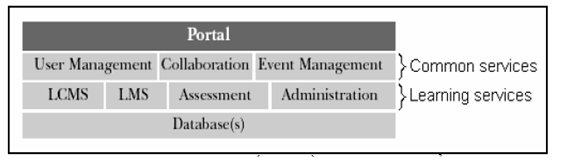
\includegraphics[width=15cm]{Chapter2/Pictures/picture21.png}
		\end{center}
		\caption{Mô hình kiến trúc nền tảng của hệ thống E-Learning}
		\label{refpicture21}
	\end{figure}
\end{center}

	Hình 2.1 mô tả mô hình kiến trúc nền của hệ thống E-Learning gồm 4 tầng liên quan với nhau là tầng cổng (Portal), tầng dịch vụ chung (Common Services), tầng dịch vụ đào tạo (Learning services) và tầng cơ sở dữ liệu (Databases). Tầng Portal chứa những giao tiếp với hệ thống. Tầng Common services chứa những dịch vụ dùng chung cho toàn hệ thống và Tầng Databases chứa cơ sở dữ liệu. Các tầng trên đều là những tầng dịch vụ thường thấy ở bất kì hệ thống nào. Phần sau đây sẽ trình bày điểm riêng của hệ thống E-Learning với các hệ thống khác, nằm ở tầng Learning Services. Tầng Learning Services gồm có:
	\begin{itemize}
		
		\item \textbf{Hệ quản trị nội dung LCMS (Learning Content Management System):} là một ứng dụng phần mềm cho phép tạo nội dung, lưu trữ, quản lý và xuất bản những nội dung đào tạo để phân phối qua mạng, LCMS cần cung cấp những khả năng mềm dẻo nhất cho việc soạn bài giảng, quản lý bài giảng,... Ngày nay có rất nhiều ứng dụng bên thứ 3 cho phép làm việc này, một số công cụ còn được thương mại hóa với độ ổn định cao.
	
		\item \textbf{Hệ quản trị đào tạo LMS (Learning Management System):} là phần mềm tự động hóa việc quản lý các sự kiện đào tạo. LMS ghi nhận các thao tác của người dùng, tạo các khoá học, phân cấp khóa học theo các danh mục khóa học và cung cấp các bản thông báo cho việc quản lý. Một hệ LMS được thiết kế để có thể kiểm soát các khoá học từ nhiều nguồn xuất bản và nhiều nhà cung cấp. Một số LMS phổ biến hiện nay và được open-source như Moodle, Sakai,...
	
		\item \textbf{Hệ thống đánh giá:} là hệ thống đánh giá khả năng của học viên đối với khóa học, sử dụng những câu hỏi kiểm tra hay các bài tổng kết, bài tập lớn,... Từ chỗ đánh giá việc học của học viên, nó cho phép chọn những bài giảng phù hợp nhất cho học viên trong một khoá học cụ thể.
	
		\item \textbf{Hệ thống quản lý:} cho phép người quản lý bao quát được tất cả các học viên, giảng viên và những người dùng của hệ thống, cho phép tổng hợp, đánh giá dễ dàng, liên tục các dữ liệu liên quan. 	
		
	\end{itemize}

	Trong những hệ thống trình bày trong tầng Learning Services thì có 2 bộ phận quan trọng nhất đó là LCMS và LMS, hai bộ phận này đảm nhận vai trò tạo nội dung và quản lý nội dung trên các hệ thống E-Learning hiện tại. Phần tiếp theo sẽ trình bày về mối quan hệ giữa 2 đơn vị này.\\

\subsubsection{Mối quan hệ LCMS và LMS}

	LCMS và LMS là khác nhau nhưng chúng phối hợp với nhau để mang lại hiệu quả hoạt động cho hệ thống E-Learning. Khi được kết hợp chặt chẽ, thông tin từ hai hệ có thể được trao đổi, chuyển giao cho nhau. Hình vẽ dưới đây thể hiện một mô hình kết hợp giữa hai hệ[2].


\begin{center}
	\begin{figure}[htp]
		\begin{center}
			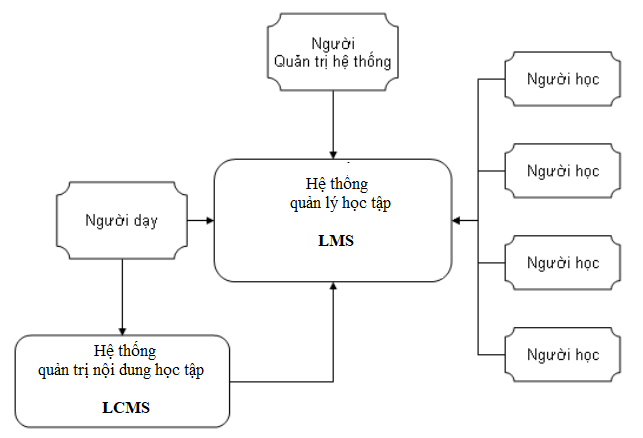
\includegraphics[width=15cm]{Chapter2/Pictures/picture22.png}
		\end{center}
		\caption{Mối quan hệ LMS và LCMS}
		\label{refpicture22}
	\end{figure}
\end{center}

	Hình 2.2 mô tả tổng quan về mối liên hệ giữa 2 đơn vị LCMS và LMS, qua đó người dạy sẽ thông qua hệ thống LCMS để tạo và quản lý nội dung sau đó đưa gói nội dung lên các hệ thống quản lý học tập như Moodle, Sakai,… Người học sẽ được cung cấp tài khoản và đăng nhập vào hệ thống, người quản trị hệ thống sẽ cung cấp các quyền truy cập vào khóa học cho người học.
	
\newpage

\section{Chuẩn SCORM}
	\subsection{Sự ra đời của SCORM}
	
	Khi E-Learning ra đời đã làm phát sinh một số vấn đề liên quan đến việc giao tiếp giữa LCMS và các LMS. Cần có 1 chuẩn đóng gói nội dung để có thể sử dụng với nhiều LMS khác nhau, nhằm giảm chi phí khi có nhu cầu đổi từ LMS này sang một LMS khác tốt hơn. Từ cơ sở để giải quyết vấn đề nêu trên, các tổ chức lớn lần lượt nêu lên các đặc tả để giải quyết như đặc tả về đóng gói nội dung, đặc tả về trao đổi thông tin giữa nội dung và hệ thống đào tạo. Các đặc tả nói trên được phát triển bởi các tổ chức khác nhau và nhằm giải quyết các vấn đề khác nhau trong E-Learning. Mặc dù được chấp nhận như các chuẩn không chính thức trong cộng đồng E-Learning, các đặc tả tồn tại riêng lẻ, không thống nhất và không có quan hệ chặt chẽ với nhau. Để phát triển E-Learning hiệu quả, chi phí thấp cần có một mô hình thống nhất các đặc tả trên lại với nhau. Như vậy, với nhu cầu cần một chuẩn đặc tả chung về việc đóng gói nội dung và giao tiếp giữa LCMS và LMS, từ đó chuẩn SCORM ra đời.

	\subsection{Khái niệm của chuẩn SCORM}
	
	SCORM (Shareable Content Object Reference Model – Mô hình tham chiếu đối tượng nội dung dùng chung) là mô hình tham khảo các chuẩn kỹ thuật, các đặc tả và các hướng dẫn có liên quan được đưa ra bởi các tổ chức khác nhau dùng để đáp ứng các yêu cầu ở mức cao của nội dung học tập và các hệ thống thông qua các từ “ilities” như sau.\\

	\textbf{Môi trường học tập dựa trên chuẩn SCORM có những khả năng sau:}\\

	\begin{itemize}
	
		\item \textit{Tính truy cập được (Accessibility):} Khả năng định vị và truy cập các nội dung giảng dạy từ một nơi ở xa và phân phối nó tới các vị trí khác.
	
		\item \textit{Tính thích ứng được (Adaptability):} Khả năng cung cấp các nội dung giảng dạy phù hợp với yêu cầu của từng cá nhân và tổ chức.
	
		\item \textit{Tính kinh tế (Affordability):} Khả năng tăng hiệu quả và năng suất bằng cách giảm thời gian và chi phí liên quan đến việc phân phối các giảng dạy.
	
		\item \textit{Tính bền vững (Durability):} Khả năng trụ vững với sự phát triển và thay đổi của công nghệ mà không phải thiết kế lại tốn kém, cấu hình lại.
	
		\item \textit{Tính khả chuyển (Interoperability):} Khả năng làm cho các thành phần giảng dạy tại một nơi với một tập công cụ hay platform và sử dụng chúng tại một nơi khác với một tập các công cụ hay platform.
	
		\item \textit{Tính sử dụng lại (Reusability):} Khả năng mềm dẻo trong việc kết hợp các thành phần giảng dạy trong nhiều ứng dụng và nhiều ngữ cảnh khác nhau.
	
	\end{itemize}


	Nhờ những khả năng trên của chuẩn SCORM mà hiện nay SCORM được sử dụng nhiều nhất khi xây dựng một bài giảng E-Learning.
	
\newpage

	\subsection{Các phiên bản của SCORM}
	
	Các phiên bản của SCORM ngày càng được hoàn thiện để thực hiện đầy đủ các yêu cầu về các tính năng. Các phiên bản SCORM đã ra đời là: SCORM 1.1, SCORM 1.2, SCORM 1.3 hay còn gọi là chuẩn SCORM 2004. \\

	Tháng 1/2004, SCORM 2004 được công bố và là phiên bản ổn định, ADL hứa hẹn rằng trong tương lai gần, sẽ không có những thay đổi lớn đối với các chuẩn hiện có. ADL chỉ tập trung vào việc mở rộng phạm vi của SCORM và bổ sung các phần mới vào tài liệu hiện tại. Sẽ có những cập nhật trong tương lai song nó sẽ không làm đảo lộn mọi thứ, chắc chắn nội dung tương thích với SCORM 2004 vẫn có thể sử dụng lại được. Hệ thống tương thích với SCORM 2004 sẽ không cần phải sửa lại toàn bộ theo phiên bản tiếp theo của SCORM. \\

	SCORM 2004 được xem là nền móng vững chắc cho sự phát triển của các nội dung và các ứng dụng liên quan tới nó.\\


	\subsection{Tổ chức đặc tả của chuẩn SCORM}
	
	SCORM là một tập hợp những chuẩn đặc tả, được tổ chức thành bốn cuốn tài liệu: SCORM Overview, SCORM CAM (SCORM Content Aggregation Model), SCORM RTE (SCORM Run-Time Enviroment) và SCORM Sequencing and Navigation[3].\\


	\textbf{a. SCORM Overview:}\\
	Cuốn sách này trình bày mục tiêu và lịch sử phát triển của hệ thống ADL và SCORM. Nó cũng là tài liệu tổng quan hướng dẫn sử dụng những cuốn sách khác của SCORM.\\
	
	\vspace{0.5cm}
	
	\textbf{b. SCORM CAM:}\\
	Cuốn sách này trình bày những nội dung như sau:
	\begin{itemize}
		\item \textit{Định nghĩa các thành phần sử dụng trong một bài học.}
		\item \textit{Đóng gói các thành phần.}
		\item \textit{Mô tả các thành phần để có thể tìm kiếm và khai phá.}
		\item \textit{Định nghĩa các luật sắp xếp cho các thành phần trong bài học.}									
	\end{itemize}


	Để thực hiện nội dung đó, SCORM CAM định nghĩa nhiệm vụ và đưa ra yêu cầu đối với việc xây dựng những tập hợp nội dung (khóa học, bài học, module,…) đồng thời đề xuất cấu trúc và tổ chức cho những tập hợp nội dung đó. SCORM CAM cũng đề cập đến những quy tắc cần tuân thủ khi tạo gói tin nội dung, cách sử dụng metadata để mô tả các thành phần trong gói nội dung nhằm phục vụ cho việc tìm kiếm, lưu trữ và sử dụng lại.\\
	\vspace{0.5cm} 
	
	\textbf{c. SCORM RTE:}\\	
	Mô tả những yêu cầu của LMS để quản lý nôi trường thực thi (xử lý thể hiện nội dung, thông tin giữa nội dung và LMS, phần tử mô hình dữ liệu chuẩn được sử dụng để chuyển thông tin đến người học).\\
	
	\vspace{0.5cm}
	
	\textbf{d. SCORM Sequencing and Navigation:}\\	
	Mô tả các thông tin điều hướng nội dung trong bài học. Hướng người học theo một kịch bản mà người biên soạn muốn[3]. Cung cấp một số mô hình điều hướng thường sử dụng như: “Linear”, “No Sequencing”, “Constraint Choice”,...	
	
	

\newpage

\subsection{Gói nội dung (Content Package) được đóng gói theo chuẩn SCORM}

	SCORM cung cấp những đặc tả một cách chi tiết về những kỹ thuật cơ bản trong E-Learning như metadata, gói nội dung và xác định cơ chế cho việc giao tiếp với nội dung học tập. Một gói nội dung trong SCORM có thể là một bài học, một khóa học hay một môn học, được đóng gói thành file .zip, sau đó import vào các LMS.\\

	Gói nội dung của SCORM được mô tả như sau:\\

\begin{center}
	\begin{figure}[htp]
		\begin{center}
			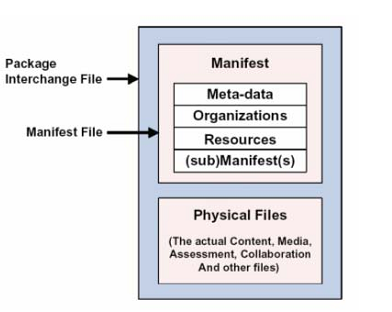
\includegraphics[width=16cm]{Chapter2/Pictures/picture23.png}
		\end{center}
		\caption{Cấu trúc của một đối tượng trong SCORM}
		\label{refpicture23}
	\end{figure}
\end{center}

\newpage

	Các thành phần có trong gói nội dung: \\
	
	\begin{itemize}
	
	\item \textbf{File imsmanifest.xml:} là file XML (imsmanifest.xml) nằm ở mức độ cao nhất đặc tả cho việc đóng gói nội dung. Nó điều hướng cho Hệ thống quản lí việc học (Learning Management System-LMS) xác định các nguồn tài nguyên được sử dụng trong bài học. Ngoài ra file này sẽ cung cấp các thông tin điều hướng nội dung theo chuẩn SCORM. Trong file này sẽ bao gồm những nội dung sau:\\

	\begin{itemize}
		\item \textbf{Meta-data}: Phần này được trình bày đầu tiên trong file imsmanifest.xml, là phần cung cấp thông tin về gói nội dung, tác giả cũng như chuẩn SCORM hỗ trợ.
	
		\item \textbf{Organizations}: Là phần tiếp theo trong file imsmanifest.xml, là thành phần chứa dữ liệu về cấu trúc nội dung trong gói. Cấu trúc này là cách sắp xếp nội dung bài học theo từng chương, từng mục. Các thông tin điều hướng các hoạt động của bài học cũng được trình bày tại đây.
	
		\item \textbf{Resources}: Phần cuối trong file imsmanifest.xml, dùng để chứa các đường dẫn đến các tài nguyên trong bài học.
	\end{itemize}


	\item \textbf{Physical Files:} Bao gồm hai thành phần, thứ nhất là các file hệ thống của SCORM và thứ hai là các file chứa nội dung bài học, các file media phục vụ cho nội dung của bài học, các file này do người biên soạn tạo ra.\\

\end{itemize}
\vspace{0.5cm}
Như vậy việc tạo một gói SCORM bao gồm các công việc:
\begin{itemize}
	\item Tạo 1 thư mục gốc để chứa các file thành phần.
	\item Tạo (copy) các file hệ thống của SCORM vào thư mục gốc.
	\item Tạo (copy) các file của bài học vào thư mục gốc.
	\item Biên tập file imsmanifest.xml cho phù hợp với các file của bài học.
	\item Đóng gói tất cả các file vào một file zip.
\end{itemize}

\subsection{SCORM Engine - Công cụ đọc nội dung theo chuẩn SCORM}
\subsubsection{6.1 Giới thiệu SCORM Cloud}
SCORM Cloud là một Hệ quản trị đào tạo (Learning Management System) trực tuyến. SCORM Cloud cung cấp một môi trường quản lý học tập trực quan, mô hình quản lý học tập này vẫn tuân theo cấu trúc đã đưa ra ở hình 2.2.\\

Với SCORM Cloud, người dạy có thể tạo nội dung học tập hoặc dùng các nội dung đã có upload lên. Những bài học này sẽ được thêm vào thư viện của người dạy, sau đó người dạy có thể theo dõi trạng thái của từng bài học khác nhau thông qua các thông số mà SCORM Cloud cung cấp như số người tham gia vào bài học này, thống kê số người hoàn thành khóa học, thời gian khóa học thường bắt đầu,... Hình 2.4 mô tả một số thông tin người dạy có thể theo dõi của khóa học hiện tại.\\

\vspace{0.5cm}

\begin{center}
	\begin{figure}[htp]
		\begin{center}
			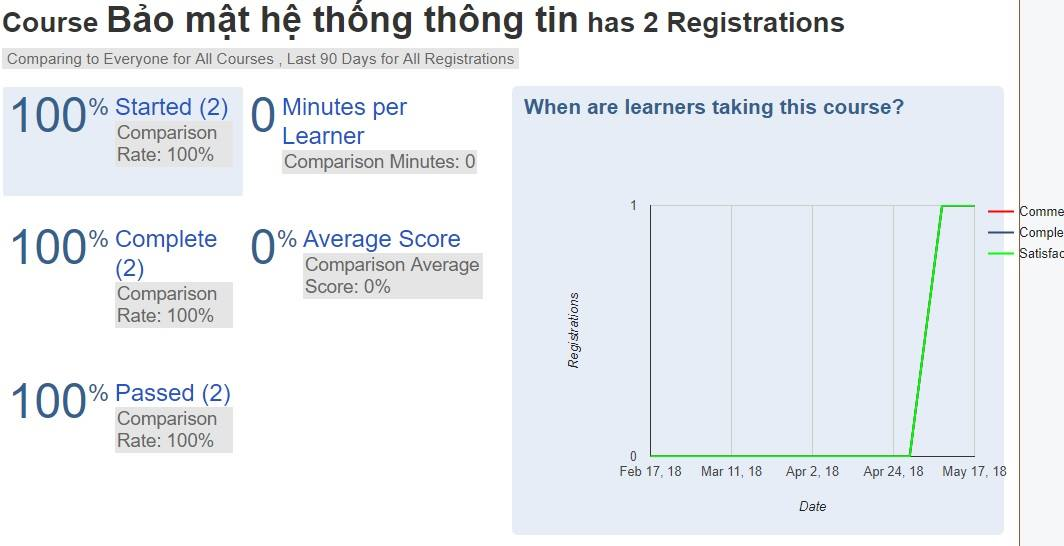
\includegraphics[width=15cm]{Chapter2/Pictures/picture24.jpg}
		\end{center}
		\caption{Thông tin một khóa học trên SCORM Cloud}
		\label{refpicture24}
	\end{figure}
\end{center}
\newpage

\subsubsection{6.2 Ưu điểm của SCORM Cloud so với các LMS khác}
SCORM Cloud hoạt động như là một dịch vụ Web nên không cần phải cài đặt, chỉ cần trình duyệt web là có thể sử dụng được. Với những Hệ quản trị đào tạo mã nguồn mở như Moodle, Sakai,... Người quản lý có thể dễ dàng tùy chỉnh thiết lập của mình, thay đổi source,... tùy vào mục đích sử dụng. Còn SCORM Cloud đã được thường mại hóa, do Rustici Softwares phân phối nên không  thể điều chỉnh giao diện quản lý theo ý người sử dụng, nhưng bù lại không cần tốn chi phí cài đặt server, tính ổn định của nó rất cao và hỗ trợ quản lý khóa học cực kỳ hiệu quả. Chỉ cần đăng ký tài khoản là có thể sử dụng các dịch vụ của SCORM Cloud. Hình 2.5 giới thiệu giao diện của người dùng trên SCORM Cloud.\\

\begin{center}
	\begin{figure}[htp]
		\begin{center}
			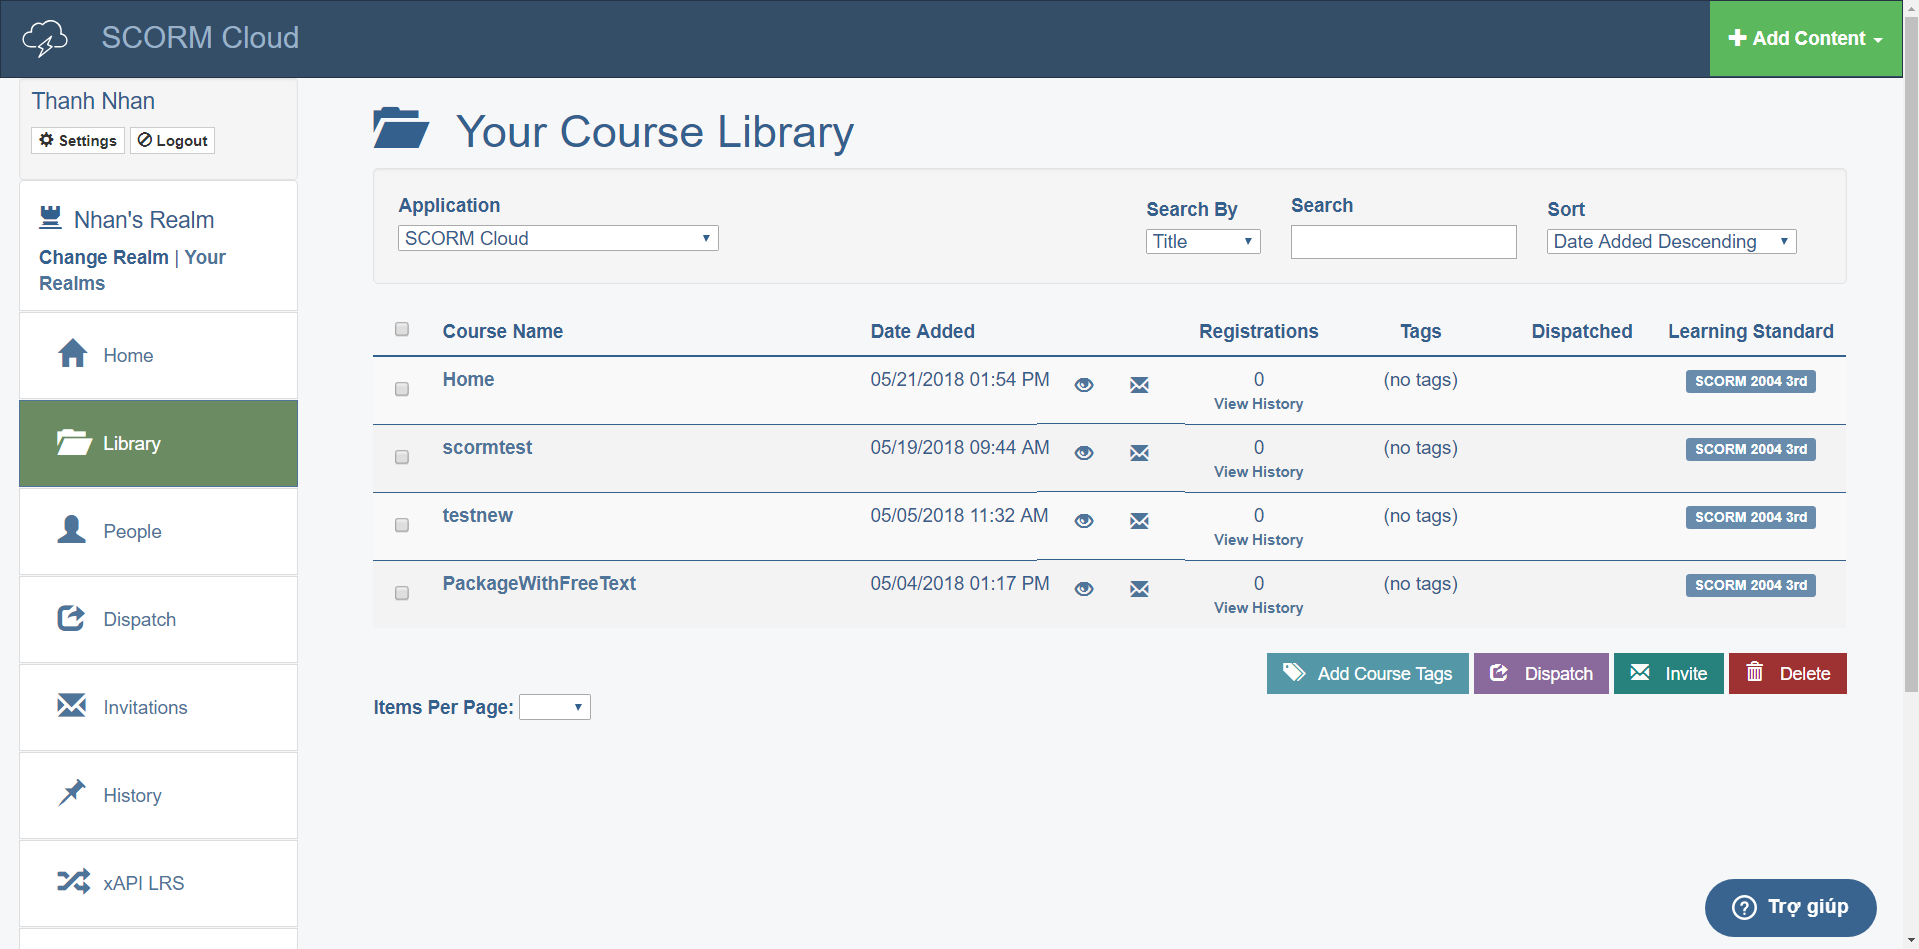
\includegraphics[width=17cm]{Chapter2/Pictures/picture25.png}
		\end{center}
		\caption{Giao diện người dùng trên SCORM Cloud}
		\label{refpicture25}
	\end{figure}
\end{center}


SCORM Cloud hỗ trợ chuẩn SCORM rất tốt, có thể nói đây là SCORM Engine mạnh nhất hiện nay. Nếu như Moodle hay Sakai bị hạn chế một số tính năng của chuẩn SCORM,  như Moodle không hỗ trợ những đặc tả Sequencing(điều hướng) của chuẩn SCORM 2004,  thì SCORM Cloud hỗ trợ đầy đủ các tính năng cho tất cả các phiên bản SCORM khác nhau, từ SCORM 1.2 đến phiên bản mới nhất SCORM 2004 phiên bản thứ 3.\\

Hình 2.6 mô tả cách sử dụng SCORM Cloud, đầu tiên người soạn thảo dùng eXe để biên soạn nội dung bài giảng, đóng gói bài giảng bằng chuẩn SCORM 2004, sau đó upload lên SCORM Cloud để nhiều học viên cùng tham gia vào bài học này.\\


\begin{center}
	\begin{figure}[htp]
		\begin{center}
			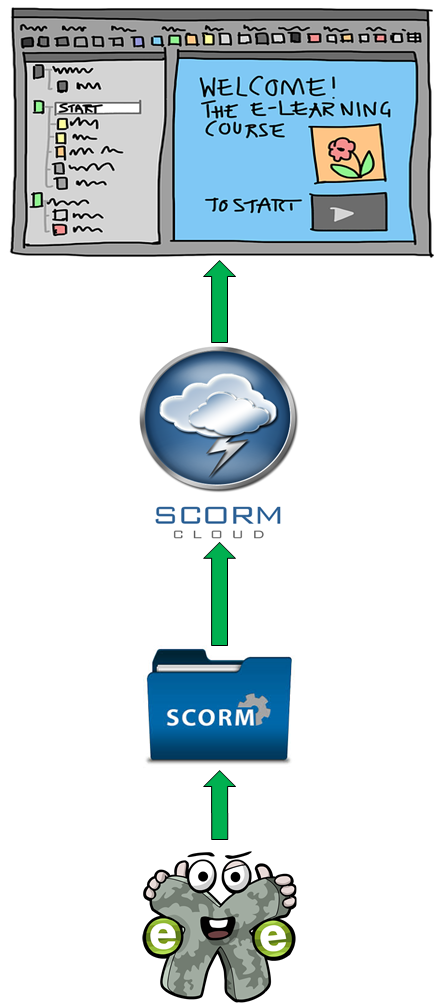
\includegraphics[width=8cm]{Chapter2/Pictures/picture26.png}
		\end{center}
		\caption{Cách sử dụng SCORM Cloud}
		\label{refpicture26}
	\end{figure}
\end{center}

\section{Công cụ eXe Learning}

\subsection{Sơ lược về hệ thống eXe Learning}
\subsubsection{1.1 Lịch sử ra đời của eXe Learning}
eXe Learning là một dự án mã nguồn mở, được tài trợ bởi chính phủ New Zealand và hai trường đại học tại New Zealand là University of Auckland và Auckland University of Technology. Dự án được bắt đầu phát triển vào năm 2007 nhưng không được nhiều thành công như mong đợi. Vào năm 2010, viện đại học INTEF (Tây Ban Nha) quyết định khởi động lại dự án với cái tên mới là “The new eXe Learning” nhưng vẫn giữ các mục tiêu ban đầu là “Free and open source”, nó là phiên bản của eXe Learning hiện tại. Phiên bản hiện tại là phiên bản 2.1.3 được phát hành vào năm 2015. Hiện tại, eXe Learning đã có một cộng đồng người dùng rộng lớn, thường xuyên đóng góp ý kiến trên diễn đàn và hệ thống hứa hẹn sẽ được hỗ trợ lâu dài.\\

\subsubsection{1.2 Giới thiệu phần mềm eXe Learning}
eXe Learning là một ứng dụng trên web, tuy nhiên khi sử dụng, máy tính không cần phải kết nối với Internet do hệ thống vận hành trên localhost server khi cài đặt, việc này sẽ giúp tiết kiệm chi phí vì không cần phải cài đặt server. Vì là ứng dụng trên web nên hệ thống có thể cài đặt trên nhiều hệ điều hành khác nhau.\\

\vspace{1cm}

\begin{center}
	\begin{figure}[htp]
		\begin{center}
			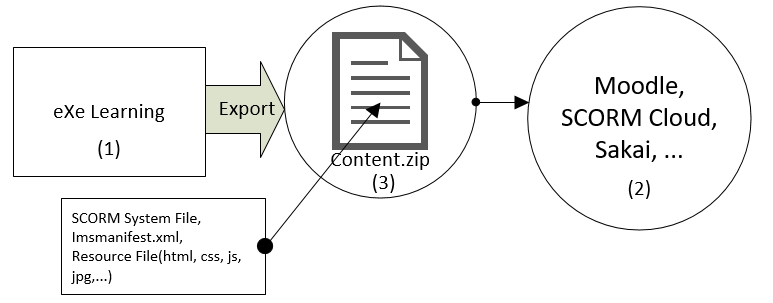
\includegraphics[width=16cm]{Chapter2/Pictures/picture27.png}
		\end{center}
		\caption{Mối quan hệ giữa hệ thống eXe Learning và LMS}
		\label{refpicture27}
	\end{figure}
\end{center}

\newpage

Hình 2.7 là tổng quan về mối quan hệ giữa hệ thống eXe Learning và LMS. (1) là công cụ thiết kế, ở đây cụ thể là eXe Learning. Người dùng sẽ sử dụng công cụ thiết kế để soạn thảo và đóng gói thành sản phẩm (3). Các sản phẩm này sẽ được upload lên các LMS để sử dụng. (2) là một số LMS thông dụng hiện nay. LMS sẽ cung cấp một công cụ gọi là SCORM Engine để đọc và xử lý thông tin trong file nội dung đã được đóng gói.\\

eXe (eLearning XHTML editor) là một công cụ với mục đích dùng để xây dựng nội dung đào tạo trực tuyến. eXe Learning cung cấp một môi trường soạn thảo bài giảng trực quan, hình 2.8 là giao diện tương tác của công cụ gồm có 3 Panel chính, Outline Panel là vùng thiết kế cấu trúc bài học, Idevice Panel là vùng lựa chọn các iDevice và Authoring Panel là vùng soạn thảo nội dung bài học. Bắt chước tính năng “wysiwig” (What You See Is What You Get), eXe cho phép người dùng xem nội dung sẽ trông như thế nào khi được xuất bản trực tuyến, hỗ trợ giáo viên tối đa trong việc thiết kế và xuất bản tài liệu học tập mà không cần có kiến thức về HTML, CSS hay XML. \\

\begin{center}
	\begin{figure}[htp]
		\begin{center}
			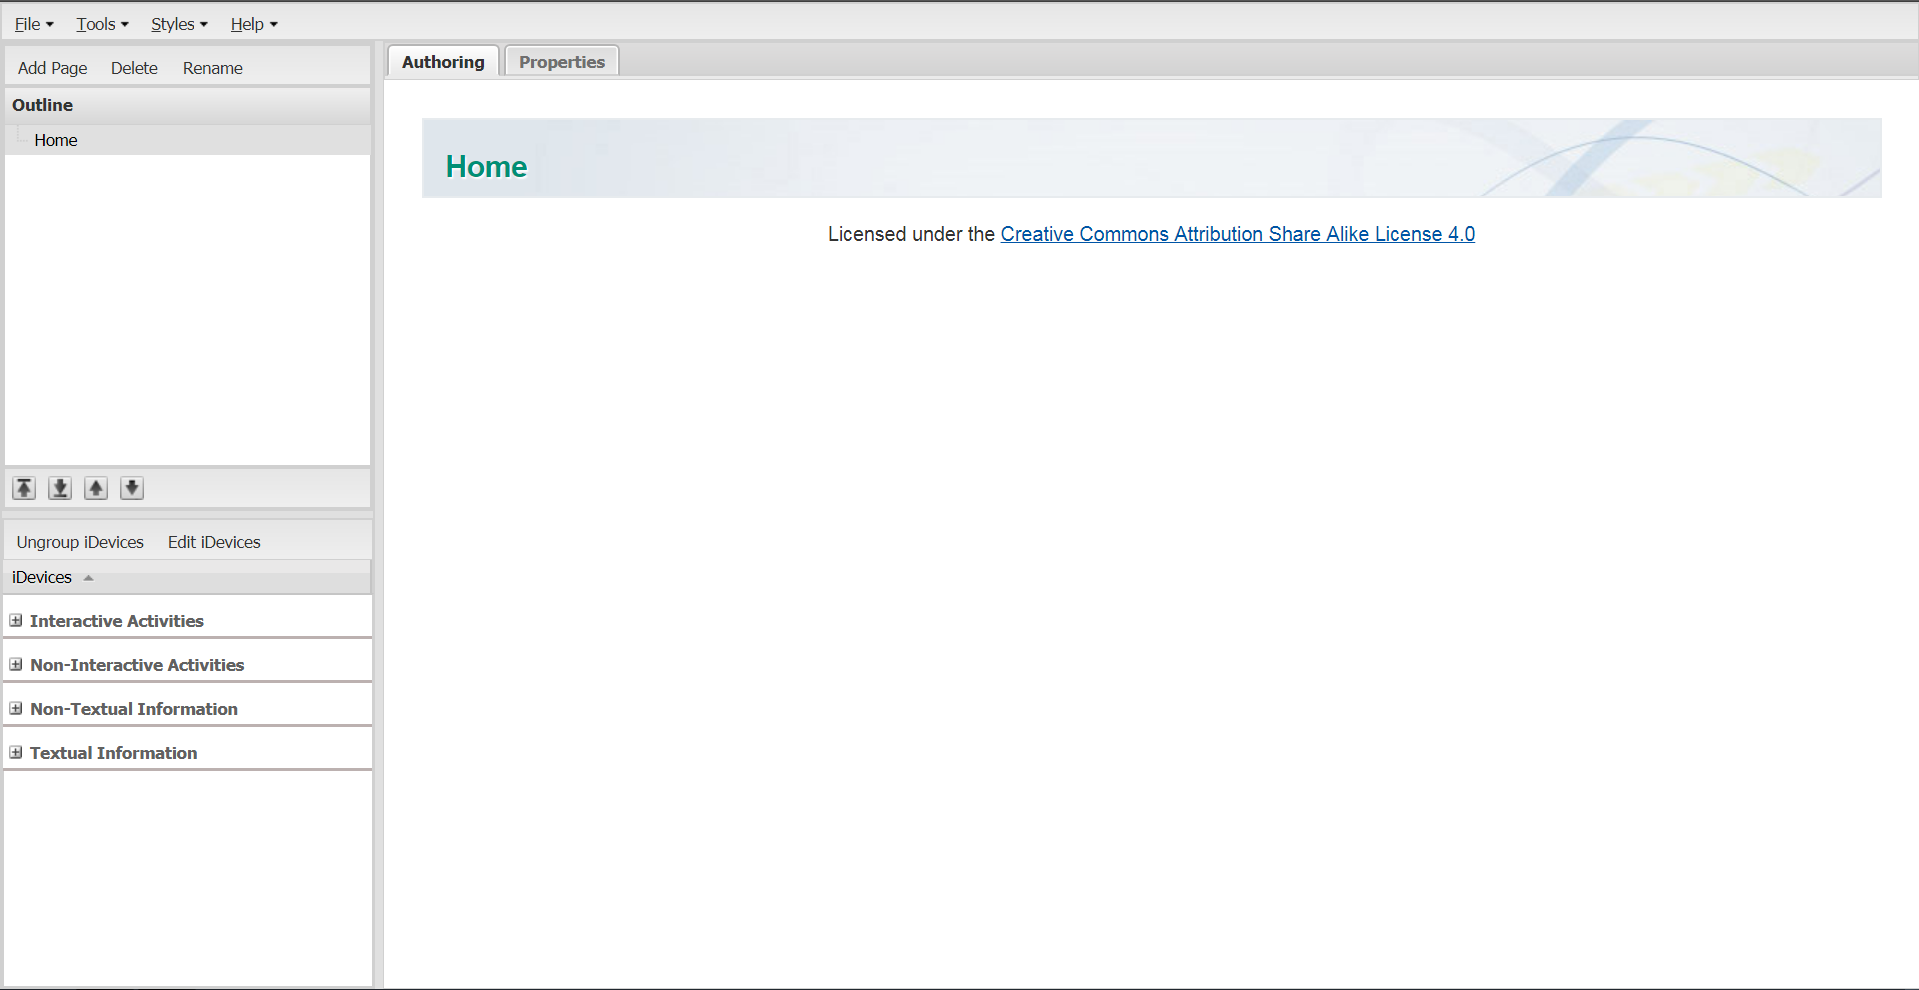
\includegraphics[width=15cm]{Chapter2/Pictures/picture28.png}
		\end{center}
		\caption{Giao diện tương tác của eXe}
		\label{refpicture28}
	\end{figure}
\end{center}	

Nội dung học tập được biên soạn và quản lý theo mô hình cây với các mức level khác nhau do người soạn thảo thiết lập trong Outline Panel. Khi soạn thảo bài học, người biên soạn cần lên một kịch bản rõ ràng, bài giảng sẽ có nhiều Topic, mỗi Topic có nhiều Section, mỗi Section có nhiều Unit được hình thành từ các trang nội dung. Một trang nội dung có thể bao gồm nhiều loại hoạt động khác nhau như câu hỏi trắc nghiệm multi-choice, case study, true-false questions, reading activity,… Các loại hoạt động này được xây dựng sẵn thành các Instruction Device (hay còn gọi là iDevice). iDevice được xem là các module được thiết kế sẵn nhằm mục đích hỗ trợ cho việc soạn thảo bài học. Hình 2.9 mô phỏng cấu trúc nội dung bài học được chia thành nhiều level khác nhau, được thiết kế trong Outline Panel và các iDevice được tích hợp sẵn trong iDevice Panel, các iDevice này được phân ra thành các nhóm như: Interactive Activity, Non-interactive activity, Textual activity,... Việc sử dụng các iDevice này sẽ tùy vào mục đích của người biên soạn.

\newpage

\begin{center}
	\begin{figure}[htp]
		\begin{center}
			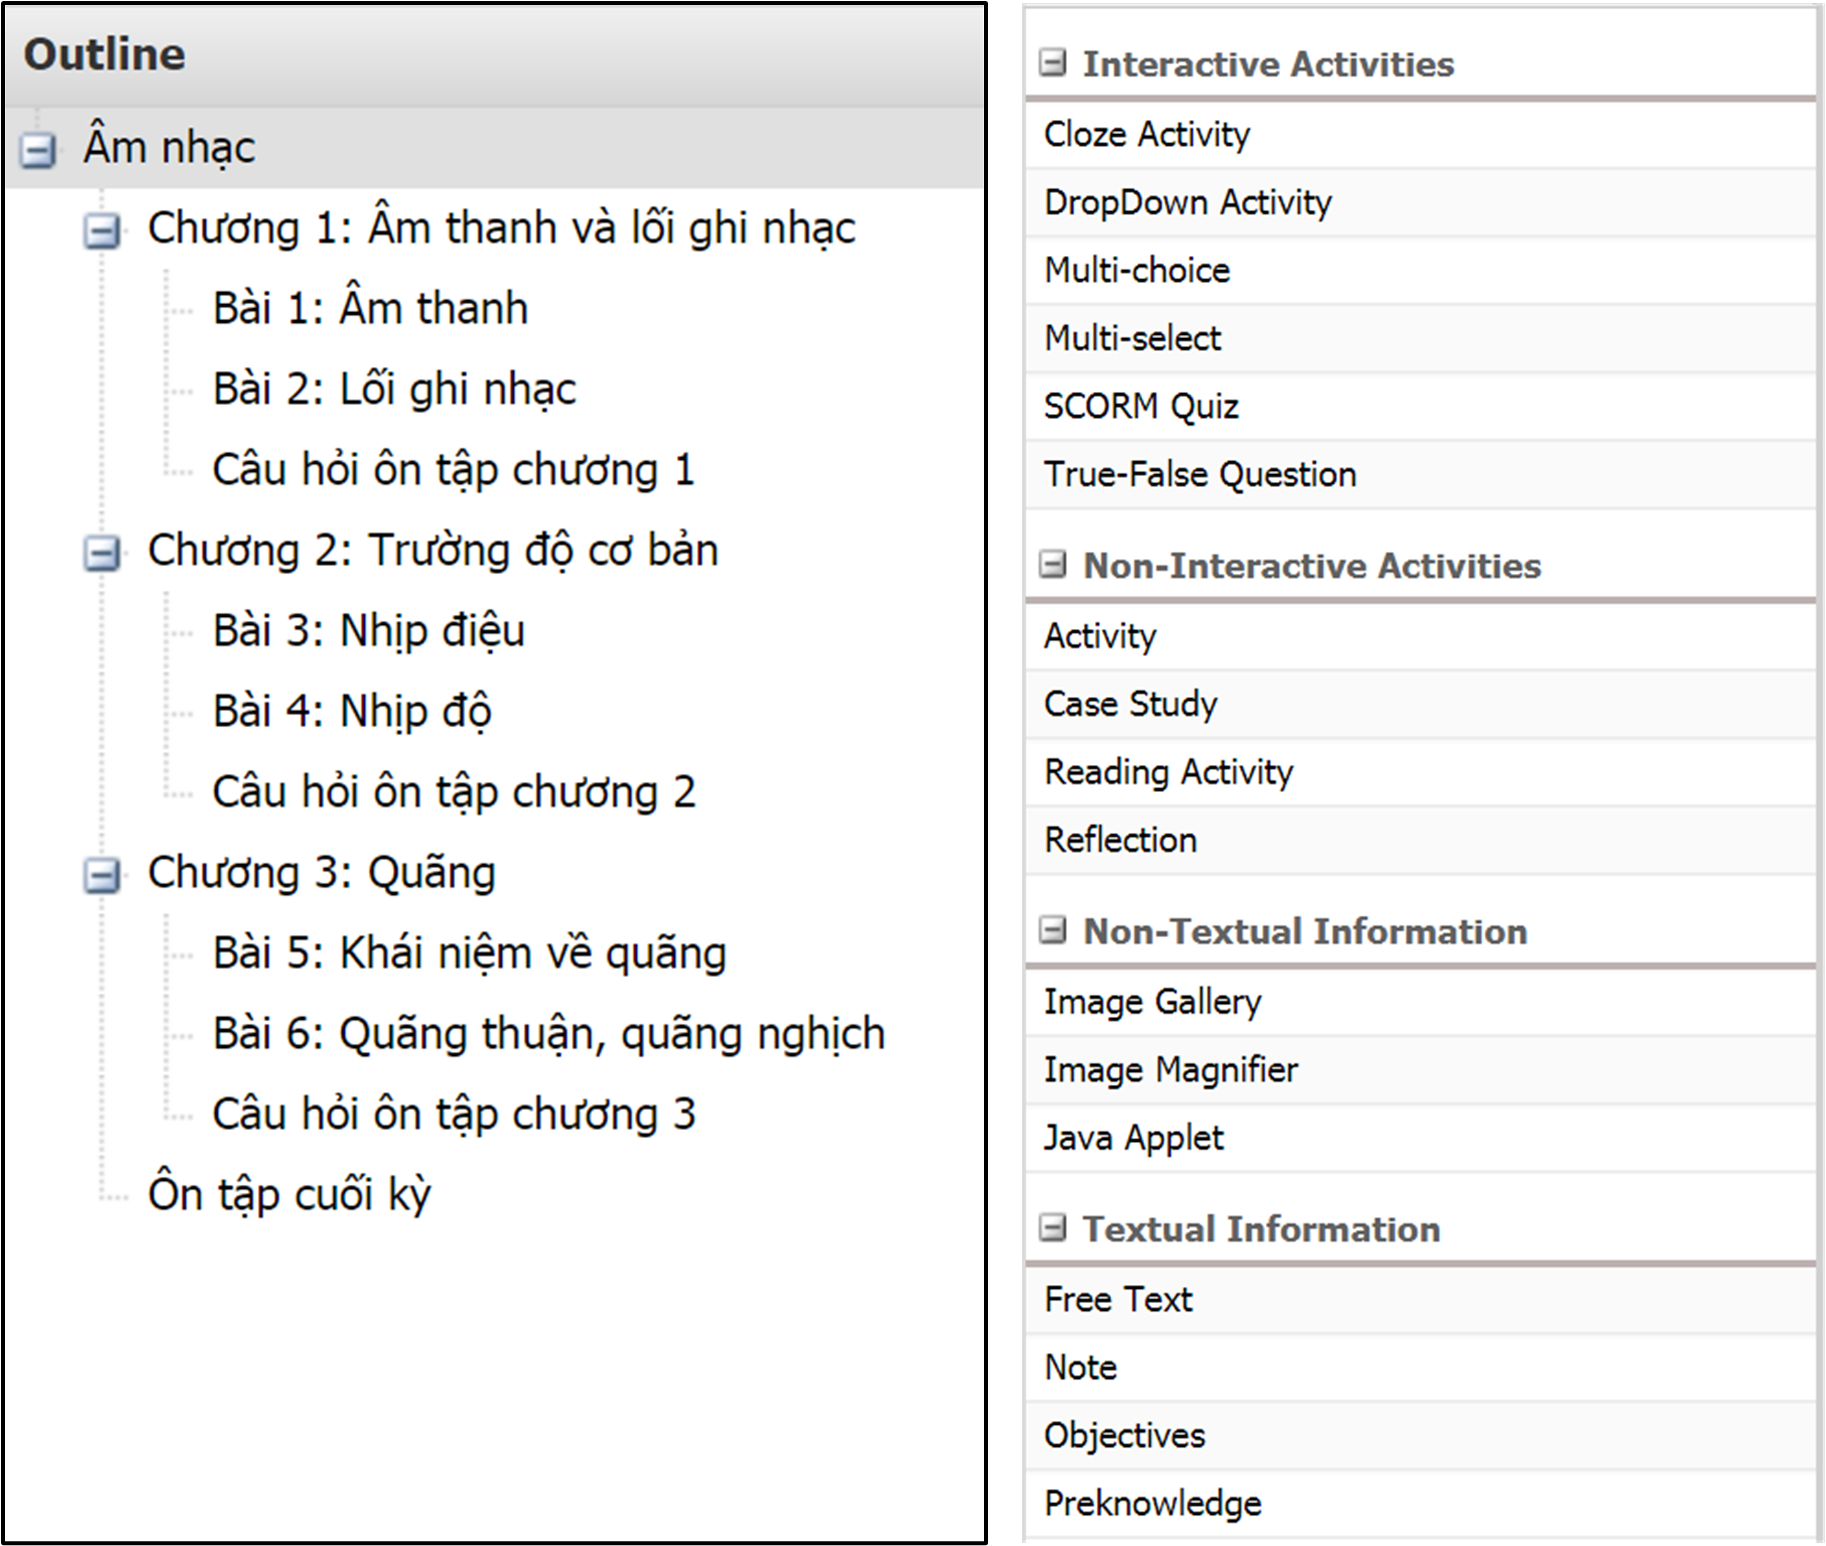
\includegraphics[width=15cm]{Chapter2/Pictures/picture29.png}
		\end{center}
		\caption{Giao diện Outline Panel và iDevice Panel}
		\label{refpicture29}
	\end{figure}
\end{center}

eXe hỗ trợ xuất ra các nội dung soạn thảo thành các định dạng khác nhau như:

\begin{itemize}
	\item Các chuẩn giáo dục: Common Cambridge, SCORM 1.2, SCORM 2004.
	\item Website.
	\item EPUB3.
	\item XLIFF.
\end{itemize}

Các gói nội dung do eXe đóng gói có thể được sử dụng lại, người soạn thảo không cần phải thiết kế lại nội dung khi chuyển từ một LMS này sang một LMS khác. Trong số các chuẩn export trên, được sử dụng phổ biến nhất là chuẩn SCORM có khả năng tương thích với hầu hết các LMS hiện nay. Trong đề tài này LMS được sử dụng để thử nghiệm là SCORM Cloud. Nội dung về SCORM Cloud đã được trình bày ở phần trên.


\subsection{Các công nghệ sử dụng trong hệ thống eXe Learning}
Mô hình Client - Server là một mô hình hết sức phổ biến hiện nay, nó là mô hình mà hầu hết các website hiện nay đang áp dụng. Hệ thống gồm 2 loại phần tử chức năng: server cung cấp 1 số dịch vụ, tài nguyên và đảm nhận vai trò xử lý các yêu cầu và trả kết quả về cho client, client là phần tử sử dụng dịch vụ bằng cách truy xuất đến server tương ứng. Hình 2.10 mô tả sơ lược cách thức hoạt động của mô hình này. Server cần phải đảm bảo có khả năng xử lý nhiều yêu cầu được gửi đến cùng một lúc.\\


\begin{center}
	\begin{figure}[htp]
		\begin{center}
			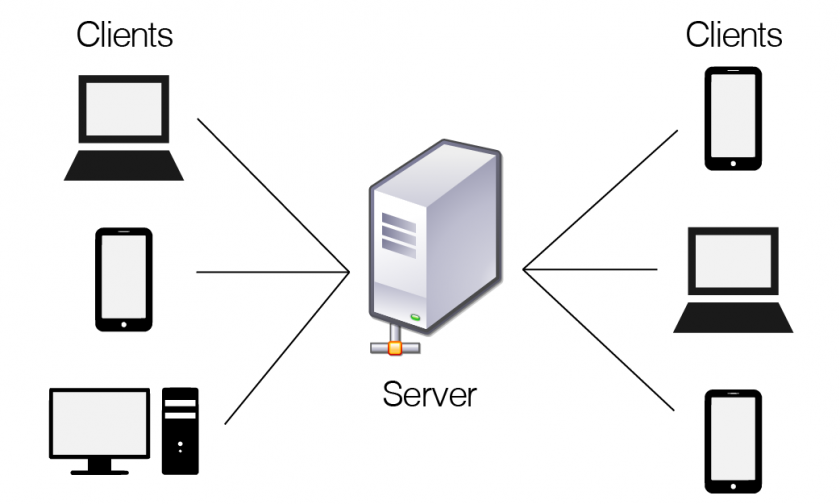
\includegraphics[width=16cm]{Chapter2/Pictures/picture210.png}
		\end{center}
		\caption{Mô hình Client – Server}
		\label{refpicture210}
	\end{figure}
\end{center}

\newpage

\textbf{Server}: Là một máy tính cho phép thực hiện yêu cầu của một hoặc nhiều người dùng từ phía client. Khi có yêu cầu từ phía người dùng, server sẽ chịu trách nhiệm xử lý và trả về kết quả cho người dùng, các kết quả này có thể là một tài nguyên nào đó nằm trên server hay một cái gì đó ví dụ như kết quả của một phép tính. Xét ở một khía cạnh khác thì server có thể được định nghĩa như một máy tính có nhiều người sử dụng vì một server phải xử lý rất nhiều các yêu cầu khác nhau từ nhiều client khác nhau, vì vậy server sẽ hoạt động tốt hơn nếu như có thể xử lý đa nhiệm, tức là các tính năng có khả năng hoạt động một cách độc lập và song song với nhau.\\

\textbf{Client}: Là máy tính chỉ được sử dụng bởi một người dùng, máy client có thể sử dụng các hệ điều hành khác nhau như Windows, Linux, MacOs,... và đóng vai trò tương tác giữa người dùng và server. Bản thân mỗi client được tích hợp nhiều tính năng và khi thông qua kết nối với server, client còn có thể sử dụng thêm những tính năng mà server cung cấp, client chỉ cần nhập các thông tin cần thiết(các tham số đầu vào) và thực hiện gửi yêu cầu lên server, sau khi server xử lý xong sẽ trả về kết quả cho client. Client và server có thể chia sẻ tài nguyên trên máy cho nhau và client được xem là người sử dụng dịch vụ do một hoặc nhiều server cung cấp.\\

eXe Learning hoạt động theo mô hình Client – Server nhưng server là localhost server, có thể xem trình duyệt web là client khi sử dụng. Exe Learning sử dụng ngôn ngữ Python bên phía server và Javascript bên phía Client. Về phía server, eXe sử dụng khung thức Twisted và Nevow để thiết lập localhost server với port mặc định là 55432, còn phía Client sử dụng khung thức ExtJS để thiết kế giao diện. Phần sau đây sẽ giới thiệu các khung thức liên quan này và các ưu nhược điểm của chúng.

\subsubsection{2.1 Khung thức máy chủ: Twisted và Nevow - Khung thức xây dựng ứng dụng mạng}

\begin{enumerate}[a.]
	\item \textit{Twisted - Khung thức mạng}\\
	Twisted là một khung thức xây dựng các ứng dụng mạng có mã nguồn mở, so với các khung thức xây dựng các ứng dụng mạng khác thì Twisted có nhiều ưu điểm nổi trội hơn như sau [4]:
	
	\begin{itemize}
		\item Thứ nhất, nó được hiện thực bằng ngôn ngữ Python, một ngôn ngữ hướng đối tượng rất mạnh, dễ đọc, dễ viết và dễ hiện thực.
		
		\item Thứ hai, vì nó hỗ trợ xử lý bất đồng bộ (Asynchronous) và lập trình hướng sự kiện(event-driven) nên Twisted có thể đảm bảo rằng ứng dụng luôn trong tình trạng có khả năng đáp ứng được nhiều request khác nhau gửi đến cùng 1 lúc, và có khả năng xử lý đồng thời các request này.
		
		\item Thứ ba, Twisted cũng cung cấp gần như đầy đủ các tính năng của nhiều loại server khác nhau tùy vào mục đích sử dụng, các loại server mà Twisted cung cấp như sau:
		\begin{itemize}
			\item \textit{twisted.web}: HTTP clients and servers, HTML templating, and a WSGI server.
			\item \textit{twisted.words}: Clients and servers for IRC, XMPP, and other IM protocols.
			\item \textit{twisted.mail}: IMAPv4, POP3, SMTP clients and servers.
			\item \textit{twisted.positioning}: Tools for communicating with NMEA-compatible GPS receivers.
			\item \textit{twisted.names}: DNS client and tools for making your own DNS servers.
			\item \textit{twisted.trial}: A unit testing khung thức that integrates well with Twisted-based code.																							
		\end{itemize}
		
		\item Cuối cùng là khả năng chia sẻ dữ liệu giữa các hệ thống không sử dụng cùng một protocol, Twisted giúp công việc đó trở nên dễ dàng hơn.
	\end{itemize}
	
	Mô hình eXe chủ yếu chỉ sử dụng module twisted.web để thiết lập local HTTP server.
	
	\item \textit{Nevow - Khung thức ứng dụng mạng}\\
	Nevow là một bộ công cụ xây dựng ứng dụng mạng được viết bằng ngôn ngữ Python do Divmod phát triển. Nevow nhằm mục đích hiện thực một kênh truyền dữ liệu 2 chiều giữa client và server mà không cần tải lại trang, thông qua việc sử dụng đối tượng XMLHttpRequest với các công nghệ như Ajax và DOM. Các dữ liệu máy chủ nhận được từ trình duyệt sẽ được lưu dưới dạng cấu trúc Dictionary của Python, còn dữ liệu mà máy chủ trả về cho trình duyệt được định dạng theo cấu trúc JSON. Nevow hoạt động tốt khi kết hợp cùng với Twisted.[5]\\
	
	\begin{center}
		\begin{figure}[htp]
			\begin{center}
				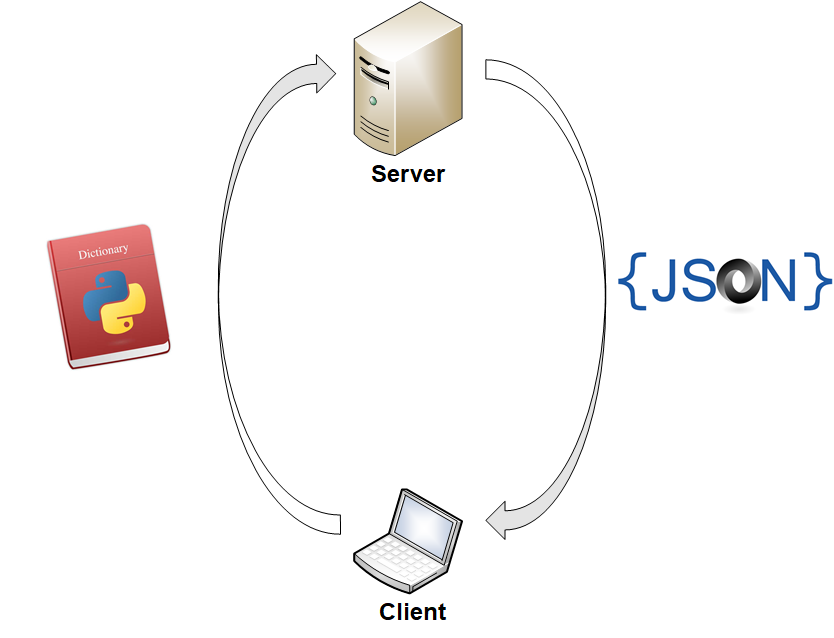
\includegraphics[width=13cm]{Chapter2/Pictures/picture211.png}
			\end{center}
			\caption{Mô phỏng quá trình hoạt động của Nevow}
			\label{refpicture211}
		\end{figure}
	\end{center}
	
	Hình 2.11 mô phỏng quá trình hoạt động của Nevow, các dữ liệu mà máy chủ nhận được từ máy khách (trình duyệt) được lưu dưới dạng cấu trúc Dictionary của Python, sau khi máy chủ xử lý dữ liệu này sẽ gửi về cho máy khách theo định dạng cấu trúc JSON.\\
	
	Tiếp theo sẽ giới thiệu khung thức mà eXe dùng để thiết kế giao diện - ExtJS.

	
\end{enumerate}

\subsubsection{2.2 Khung thức máy khách: Ext JS - Khung thức xây dựng giao diện của Javascript}
Ở phía máy khách, Exe Learning sử dụng ExtJS để thiết kế giao diện[6]. ExtJS là một Khung thức xây dựng giao diện của Javascript được dùng để thiết kế giao diện người dùng rất phong phú và thân thiện, sử dụng các công nghệ như AJAX, DOM và DHTML, do đó các ứng dụng ExtJS có tính tương tác rất cao. Ngoài ra ExtJS còn có khả năng tương tác tốt với Jquery[7]. 

Sau đây là một số đặc điểm của ExtJS:

\begin{itemize}
	
	\item Hỗ trợ đa trình duyệt và điện thoại:
	\begin{itemize}
		\item \textit{Đây là đặc điểm chung của rất nhiều các khung thức lớn có}.
		\item \textit{Được sử dụng để phát triển giao diện trên điện thoại}.
	\end{itemize}
	
	\item Phù hợp với:
	\begin{itemize}
		\item \textit{Những ứng dụng có yêu cầu giao diện đa dạng}.
		\item \textit{Làm ứng dụng trang đơn}.
		\item \textit{Mạnh mẽ với việc hỗ trợ rất nhiều dạng biểu đồ khác nhau, người phát triển không cần sử dụng thêm các công cụ khác để vẽ}.
	\end{itemize}
	
	
	\item Hỗ trợ các mô hình kiến trúc thông dụng:
	\begin{itemize}
		\item \textit{Từ bản ExtJS 4, nó hỗ trợ cả mô hình MVC (Model-View-Controller) và MVVM (Model-View-ViewModel)}.
		\item \textit{Hỗ trợ thao tác trực tiếp với DOM}.
	\end{itemize}
	
	\item Testing:
	\begin{itemize}
		\item \textit{Không hỗ trợ test tự động nhưng có thể thực hiện điều này bằng việc sử dụng thêm các công cụ hỗ trợ test ở level cao hơn}.
		\item \textit{Trong hiện thực đề tài này, nhóm sử dụng Selenium để test chức năng sau khi hiện thực}.
	\end{itemize}
	
	\item Programming:
	\begin{itemize}
		\item \textit{Hỗ trợ mô hình Object-oriented(hướng đối tượng) và Event-driven(hướng sự kiện)}.
	\end{itemize}
	
\end{itemize}

\subsection{Kiến trúc của eXe Learning}
\subsubsection{3.1 Kiến trúc hệ thống eXe Learning}

\paragraph{Mô hình hệ thống – Client Server\\}

Hệ thống eXe Learning được xây dựng là một ứng dụng web (Web Application), thiết kế dựa trên mô hình Client-Server đã được trình bày ở trên, xử lý các yêu cầu gửi tới máy chủ thông qua giao thức HTTP (request và response). Hệ thống sử dụng ngôn ngữ lập trình Python ở phía Server và JavaScript ở phái Client. Khi khởi động, hệ thống thiết lập một localhost server với port 8081 và nhận request từ brower gửi về.[8]

\begin{center}
	\begin{figure}[htp]
		\begin{center}
			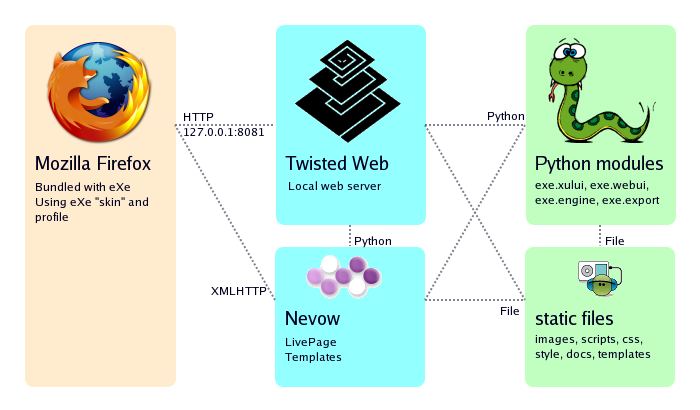
\includegraphics[width=10cm]{Chapter2/Pictures/picture212.png}
		\end{center}
		\caption{Kiến trúc vận hành của eXe}
		\label{refpicture212}
	\end{figure}
\end{center}

Hình 2.12 mô tả cụ thể cách thức hoạt động của hệ thống eXe Learning, mô-đun Twisted Web tạo HTTP localhost server với port cố định 8081 và nhận request. Tiếp theo là việc thiết lập một kênh trao đổi đảm nhận việc xử lý dữ liệu gửi và dữ liệu nhận giữa browser và server. Hệ thống sử dụng khung thức Nevow để đảm nhiệm vai trò trên, xử lý các event và tương tác giữa browser và server. Từ các request gửi về server, hệ thống sẽ phân tích yêu cầu này và gửi yêu cầu đến các module liên quan để xử lý và trả kết quả về cho browser. Các Python modules là các thành phần của phía server nhằm mục đích để xử lý các yêu cầu khác nhau, bao gồm các module giao diện đồ họa, các module đảm nhận việc đóng gói dữ liệu,... Các Static file là các resource file phục vụ cho việc thiết kế giao diện đồ họa. Người dùng sẽ sử dụng trình duyệt web, tạo kết nối tới localhost server.

\subsubsection{3.2 Kiến trúc phần mềm eXe Learning}
Như đã trình bày ở phần trên, phần mềm eXe được viết chủ yếu bằng Python ở phía server và được hiện thực thành nhiều module với các chức năng khác nhau, cụ thể được thể hiện thông qua Class Diagram sau.[9]

\begin{center}
	\begin{figure}[htp]
		\begin{center}
			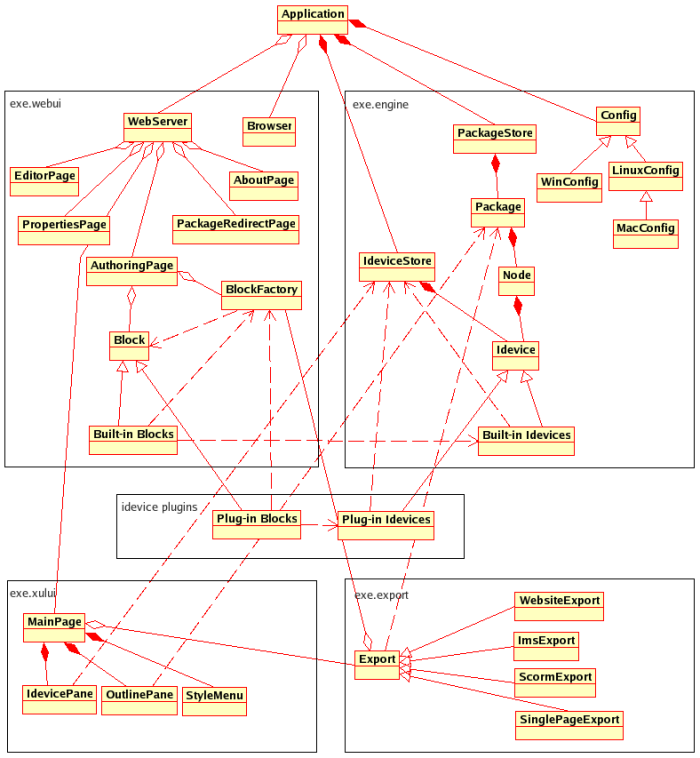
\includegraphics[width=10cm]{Chapter2/Pictures/picture213.png}
		\end{center}
		\caption{Class Diagram của phần mềm eXe}
		\label{refpicture213}
	\end{figure}
\end{center}

\newpage

Hình 2.13 là Class Diagram của eXe, mô tả tổ chức của hệ thống với hàm main của eXe nằm ở Class Application và có các modules khác nhau đảm nhận các chức năng khác nhau [10], cụ thể như sau:

\begin{itemize}
	\item \textbf{Exe.webui}: Gồm 2 Class quan trọng là WebServer và Browser. WebServer với chức năng chính là tạo port trống, sau đó khởi động các dịch vụ của server bằng các phương thức thừa kế từ twisted. Browser với chức năng chính là tìm browser mặc định của hệ điều hành và khởi động với các thiết lập từ Webrowser.
	
	\item \textbf{Exe.engine}: Module này định nghĩa các cấu trúc được sử dụng trong hệ thống như cấu trúc của một package, cấu trúc của một bài học, cấu trúc của một Block, cấu trúc của một iDevice,… Các phương thức xử lý trên chúng cũng như các phương thức xử lý dùng chung đều được định nghĩa trong module này.
	
	\item \textbf{Exe.jsui}: Module này cung cấp các phương thức xử lý request về việc render giao diện và handle các event thao tác trên giao diện. Giao diện eXe sẽ gồm 3 panel chính được mô tả như hình 2.8 và 2.9.
	
	\item \textbf{Exe.Export}: Module này cung cấp các phương thức xử lý yêu cầu đóng gói thành các định dạng khác nhau bao gồm các chuẩn Education Export là SCORM 1.2, SCORM 2004, Common Cartridge, các định dạng website Export là Single Page, Zip File, Self-contain Foder, các định dạng khác là Text File, XLIFF, EPUB3.
	
	\item \textbf{Idevice Plugins}: eXe cung cấp một công cụ tự thiết kế iDevice riêng từ các thành phần có sãn, nhưng các thành phần này bị hạn chế về số lượng nên các iDevice được thiết kế theo công cụ này gần như không có sự khác biệt so với các iDevice có sẵn. Các iDevice này sẽ được lưu trong dữ liệu cục bộ trên máy tính.									
\end{itemize}



\section{Công cụ kiểm thử sản phẩm}

\subsection{Sơ lược về kiểm thử tự động}


Kiểm thử tự động là việc sử dụng các công cụ để thực hiện các testcase một cách tự động với dữ liệu đầu vào và đầu ra đã được xác định.

Kiểm thử tự động được sử dụng khi: 
\begin{itemize}
	\item Các trường hợp kiểm thử được thực hiện lặp đi lặp lại để đảm bảo tính năng của phần mềm hoặc sản phẩm.
	\item Thực hiện ở các trường hợp mà kiểm thử thủ công khó thực hiện.
	\item Các trường hợp kiểm thử cần tốn nhiều thời gian.
\end{itemize}


Kiểm thử tự động được sử dụng trong các giai đoạn kiểm thử:
\begin{itemize}
	\item Unit Testing (Kiểm thử đơn vị).
	\item Integration Testing (Kiểm thử tích hợp).
\end{itemize}


Những ưu điểm và nhược điểm của việc kiểm thử tự động:
\begin{itemize}
	\item \textbf{Ưu điểm}: Kiểm thử tự động sử dụng các công cụ có thể ghi lại bộ kiểm tra này và phát lại nó theo yêu cầu. Tiết kiệm thời gian kiểm thử. Tự động hóa không cần can thiệp của con người nên có thể chạy tự động kiểm tra mà không cần giám sát. Tự động tăng tốc độ thực hiện kiểm tra. Tự động hóa giúp tăng phạm vi kiểm tra. Kiểm tra bằng tay có thể trở nên nhàm chán và do đó dễ bị lỗi. Cải thiện độ chính xác. Nhanh hơn so với kiểm tra thủ công.
	\item \textbf{Nhược điểm}: Các công cụ kiểm thử tự động mặc dù rất thuận tiện về nhiều phương diện nhưng thực tế dù như thế nào đi chăng nữa thì nó cũng không phải là một công cụ có thể thay thế hoàn toàn quá trình kiểm thử. Để thực hiện các thiếp lập tự động thì vẫn cần có con người, phải bỏ công sức, tiền bạc và thời gian. Mất thời gian và công sức để tạo mới và chỉnh sửa script test. Mất chi phí cho các các công cụ tự động hóa như phí bản quyền, bảo trì, tìm hiểu, giáo dục.\\
\end{itemize}

Trong luận văn này, nhóm sử dụng công cụ kiểm thử tự động là Selenium. Phần sau sẽ giới thiệu về Selenium và một số thành phần của nó.


\subsection{Tổng quan về Selenium}
\subsubsection{Lý thuyết về Selenium}

Selenium là một bộ công cụ kiểm thử tự động mã nguồn mở, dành cho các ứng dụng web, hỗ trợ hoạt động trên nhiều trình duyệt và nền tảng khác nhau như Windows, MacOS, Linux,... Với Selenium, bạn có thể viết các testscript bằng các ngôn ngữ lập trình khác nhau như Java, PHP, C\#, Ruby, Python hay thậm chí là Perl,... [11]\\

Selenium được sử dụng để tự động hóa các thao tác với trình duyệt, hay dễ hiểu hơn là nó giúp giả lập lại các tương tác trên trình duyệt như một người dùng thực sự. Ví dụ bạn có thể lập trình để tự động bật trình duyệt, mở liên kết, nhập dữ liệu, hay lấy thông tin của trang. Với selenium bạn có thể làm được rất nhiều thứ. Hơn thế nữa, bạn cũng có thể sử dụng, tùy biến để tận dụng tối đa sức mạnh của nó. Ngoài mục đích sử dụng trong kiểm thử, bạn có thể tự xây dựng một project để tự động hóa những công việc nhàm chán, lặp đi lặp lại của mình.\\


\subsubsection{Các thành phần của Selenium}
Selenium là một khái niệm chung về một bộ phần mềm được sử dụng trong tự động hóa, mỗi loại trong đó đáp ứng một yêu cầu kiểm thử khác nhau. Về cơ bản thì Selenium có 4 thành phần:

\begin{itemize}
	\item \textbf{Selenium IDE}: Selenium Integreted Development Environment (IDE), là một plug-in trên trình duyệt FireFox, ta có thể sử dụng để ghi lại và thực hiện lại các thao tác đó theo một quy trình hay một testcase nào đó, là khung thức đơn giản nhất và dễ học nhất trong bộ Selenium.
	
	\item \textbf{Selenium RC}: Selenium RC làm việc theo cách mà thư viện client có thể giao tiếp với Selenium RC Server thông qua mỗi Selenium Command để thi hành. Sau đó Server thông qua Selenium Command tới trình duyệt sử dụng các lệnh Selenium-Core Javascript. Các trình duyệt thực thi Selenium command sử dụng trình thông dịch Javascript của nó.
	
	\item \textbf{Selenium WebDriver}: Selenium WebDriver gửi lệnh khởi chạy và tương tác trực tiếp tới các trình duyệt mà không cần thông qua một server như Selenium RC.
	
	\item \textbf{Selenium Grid}: Selenium Hub dùng để khởi chạy nhiều các test thông qua các máy và các trình duyệt khác nhau tại cùng một thời điểm.
\end{itemize}
Trong luận văn này, nhóm sử dụng công cụ Selenium WebDriver để kiểm thử cho eXe nên sẽ đi sâu vào công cụ này.

\subsection{Giới thiệu Selenium WebDriver}
\subsubsection{Công cụ Selenium WebDriver}

Selenium WebDriver là công cụ tự động được sử dụng nhiều nhất trong bộ công cụ Selenium, là một trong những công cụ phổ biến nhất cho Web UI Automation (Kiểm thử giao diện trang Web tự động). Nó là một thư viện mã nguồn mở, cho phép chúng ta sử dụng nhiều ngôn ngữ lập trình khác nhau như Javam .NET, PHP, Python,... để thiết kế testcase. Đồng thời nó cũng tương tác với rất nhiều trình duyệt Web khác nhau.[12]

\subsubsection{Ưu điểm của Selenium WebDriver}

\begin{itemize}
	\item Người dùng có thể dùng miễn phí.
	
	\item Selenium WebDriver cho phép chúng ta sử dụng một trong số các ngôn ngữ lập trình như HTML, Java, .Net, Perl, Ruby,... để tạo kịch bản test (TestCase) kết hợp với sử dụng các điều kiện, vòng lặp,... khiến cho testscript trở nên chính xác hơn.
	
	\item Selenium WebDriver được phát triển tốt hơn để hỗ trợ cho các trang web động (Những trang web mà phần tử trong nó có thể thay đổi ngay cả khi trang đó không được tải lại). Mục đích của WebDriver là hỗ trợ cho các vấn đề về kiểm thử web-app hiện nay.
	
	\item Kiến trúc của Selenium WebDriver đơn giản hơn rất nhiều so với các công cụ Selenium khác. Selenium WebDriver làm việc trực tiếp với trình duyệt ở mức độ hệ điều hành, nó như một người trung gian để chuyển lệnh từ testcase của mình lên trình duyệt, do đó tốc độ của nó sẽ rất nhanh. Hình 2.4 mô tả kiến trúc của Selenium WebDriver, qua đó thể hiện Selenium WebDriver đóng vai trò như người dùng làm việc trực tiếp với browser.
	
	\item Tốc độ: Khi so sánh với các công cụ khác trong bộ Selenium, WebDriver là công cụ nhanh nhất trong số tất cả do tương tác trực tiếp từ hệ điều hành tới trình duyệt. 
\end{itemize}


\begin{center}
	\begin{figure}[htp]
		\begin{center}
			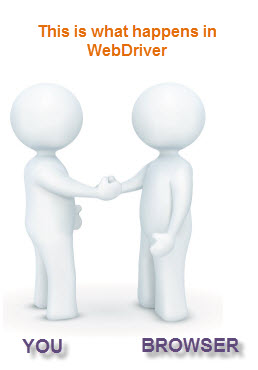
\includegraphics[width=10cm]{Chapter2/Pictures/picture214.jpg}
		\end{center}
		\caption{Kiến trúc của Selenium WebDriver [6]}
		\label{refpicture214}
	\end{figure}
\end{center}


Hình 2.14 mô tả cách làm việc của Selenium WebDriver, lúc này Selenium WebDriver đóng vai trò như người dùng, có nhiệm vụ tương tác tự động với Browser.

\newpage

\subsubsection{Một số ưu nhược điểm của Selenium WebDriver}
\begin{itemize}
	
	\item \textbf{Ưu điểm:}
	
	\begin{itemize}
		\item Giao tiếp trực tiếp với trình duyệt nên tốc độ sẽ rất nhanh.
		\item Tương tác với trình duyệt giống như thao tác của một người dùng thật.
		\item Tốc độ nhanh hơn so với các công cụ Selenium khác.
		\item Thao tác dễ dàng hơn với các phép tính toán logic hay các điều kiện phức tạp.
	\end{itemize}
	
	\item \textbf{Nhược điểm:}
	
	\begin{itemize}
		\item Cài đặt khá phức tạp.
		\item Đòi hỏi người dùng phải có kĩ năng lập trình.\\
	\end{itemize}
\end{itemize}

\subsubsection{Các trình duyệt hỗ trợ Selenium WebDriver}

\begin{center}
	\begin{figure}[htp]
		\begin{center}
			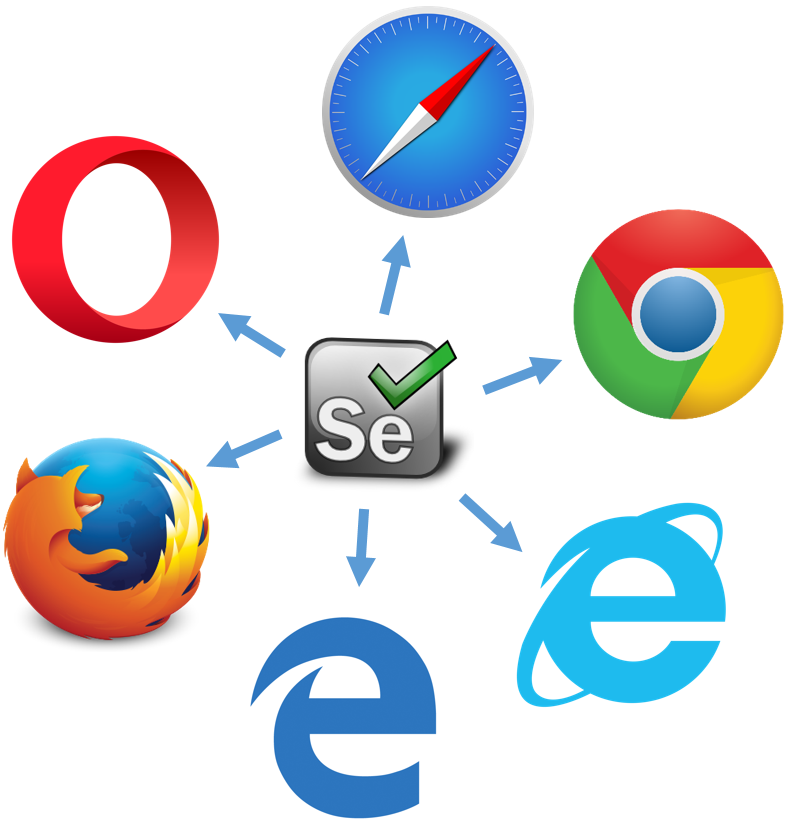
\includegraphics[width=13cm]{Chapter2/Pictures/picture215.png}
		\end{center}
		\caption{Các trình duyệt Selenium WebDriver hỗ trợ hiện nay}
		\label{refpictute215}
	\end{figure}
\end{center}

Selenium WebDriver được hỗ trợ trên rất nhiều các trình duyệt khác nhau. Do đó để sử dụng Selenium WebDriver thì chỉ cần một tập lệnh Selenium và một trình duyệt là đủ. Hình 2.15 thể hiện các trình duyệt hiện nay mà Selenium WebDriver hỗ trợ.
















